%Experiment 1-2

\chapter{Uncertainty and Error}
\label{chap:excel2}
\section{Introduction}

The purpose of this lab is to allow time to practice using the tools you were introduced to last week, while also familiarizing yourself further with Microsoft Excel, which will help you greatly throughout the year. You will complete a few exercises and one experiment, demonstrating how we can use the principles of error analysis to analyze different sets of data. The issues and techniques are important in order to arrive at accurate conclusions in any field in which it is necessary to understand not just numerical results, but the uncertainties associated with those results. \myskip

If you wish to use your personal laptop and have not already acquired a copy of Excel, you can download a copy with your student email address from
\href{https://products.office.com/en-us/student?ms.officeurl=getoffice365}{Office 365 Education}\footnote{https://products.office.com/en-us/student?ms.officeurl=getoffice365}. However, this will not be absolutely necessary since computers are provided in the laboratory. Please note the sections introducing new Excel tools pertain to the newest version of Excel. If you are using a personal computer with a different version of Excel, you are responsible for adapting the instructions to your version of Excel.

\section{Theory}

It is highly recommended that you look back on some of the lessons taught in last week's section. This lab will simply be an extension of those ideas.

\subsection{Working With Excel}
\subsubsection{Plotting with Excel}

An important set of data analysis tools in Excel are plotting and linear fit functions. You will need to plot and fit data many times throughout this lab course, so make sure you are familiar with this section. Below is a walkthrough of plotting and fitting a set of data with error in excel.
\begin{enumerate}
\item Before plotting, you need to have 4 columns with data: x data, y data, x error data, and y error data. Make sure you have entered the information into excel.
\item First select your x data and y data (you can select multiple boxes in excel by holding down the ctrl button while selecting). Make sure to select your x data first or your x and y axes will be switched.
\item Choose the subheading ``insert", then ``Scatter", then ``Scatter with straight lines and markers". Now your x and y data should be plotted without error bars (see figure \ref{fig:excel1}).

\begin{figure}[h!]
\centering
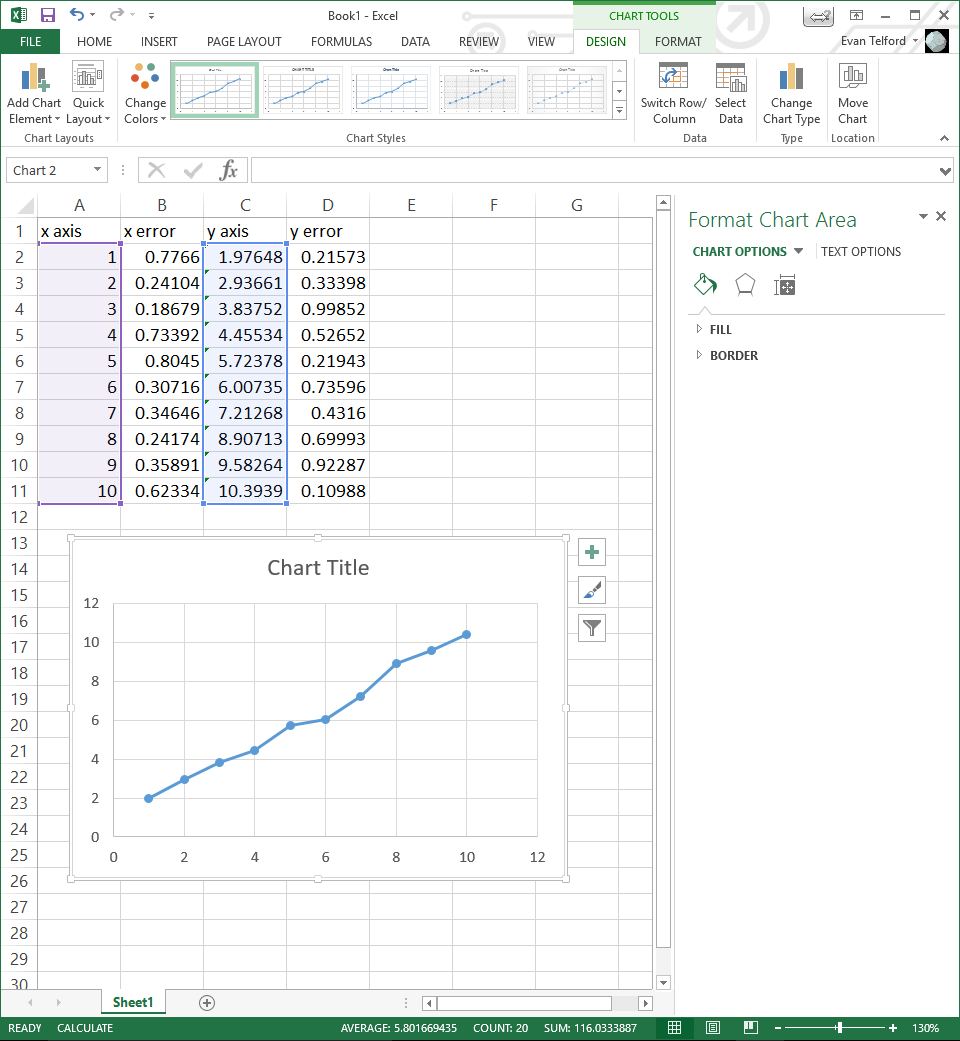
\includegraphics[height=0.4\textheight, width=0.7\textwidth]{./Exp1-2/pic/image4.png}
\caption{Selecting x and y data and creating a lined scatter plot in excel.}
\label{fig:excel1}
\end{figure}

\item To include error bars select your chart, then click the ``plus" marker on the top right of the chart. Check the box titled ``error bars". Now some basic error bars should appear on the plot. These are not based on the error bar data in your excel document, they are standard error bars.
\item To change them so they match your error bar data, select the x axis error bars on your chart, and format the error bars by clicking the ``Custom" selection, then ``specify value".
\item It should now prompt you for positive error values and negative error values. Delete ``$\{1\}$" from the two boxes, and select your error bars using the cursor. Your chart will now have the correct error bars (see figure \ref{fig:excel2}).

\item Repeat steps 5-6 for your y data.
\item To linear fit your data, right click on your data in the plot and select ``Add Trendline". Check the ``Linear", ``Display Equation on chart", and ``Display R-square value on chart" boxes.
\item Now the slope, intercept, and R squared values will be displayed on your chart. R squared is a measure of how well the line fits your data. It should be close to $1$ and at the very least greater than $0.9$.
\end{enumerate}

\begin{figure}[h!]
\centering
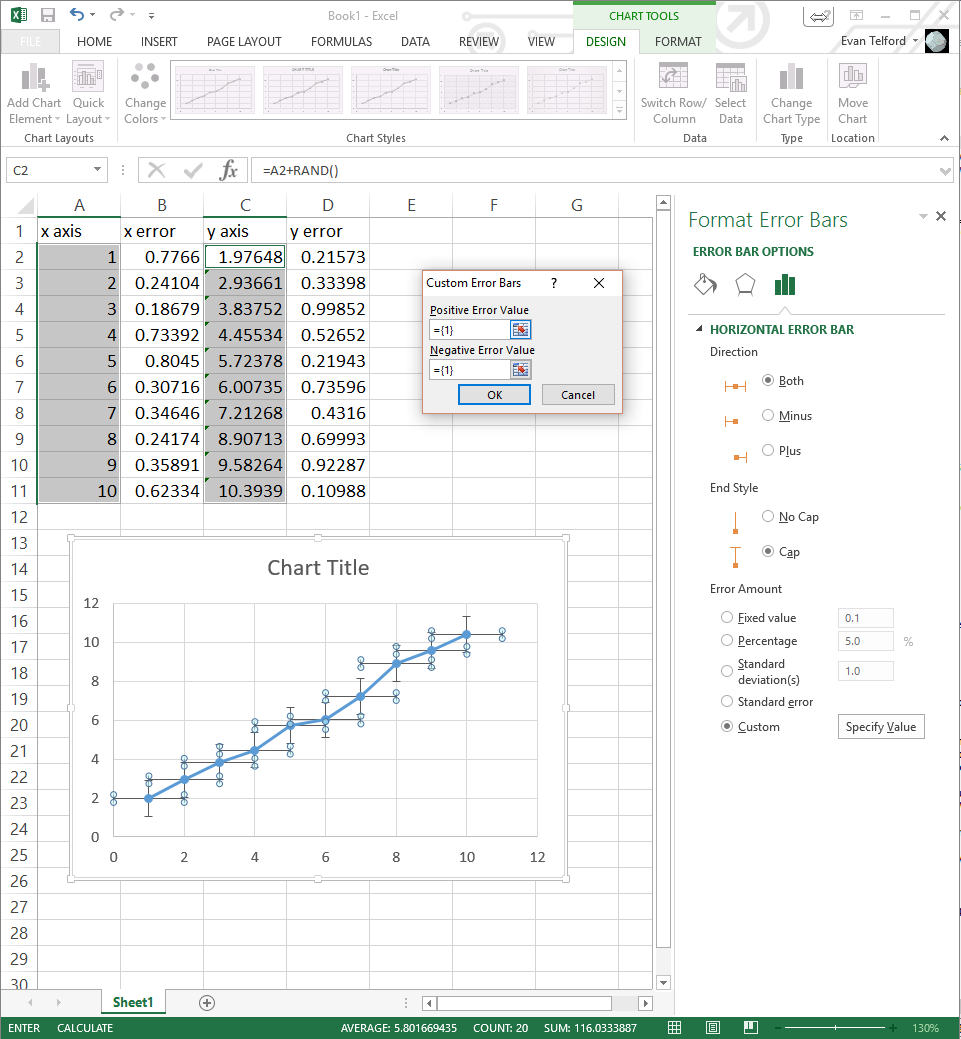
\includegraphics[height=0.4\textheight, width=0.7\textwidth]{./Exp1-2/pic/image5.png}
\caption{Using your own data set to create x and y error bars in excel.}
\label{fig:excel2}
\end{figure}

\begin{figure}[h!]
\centering
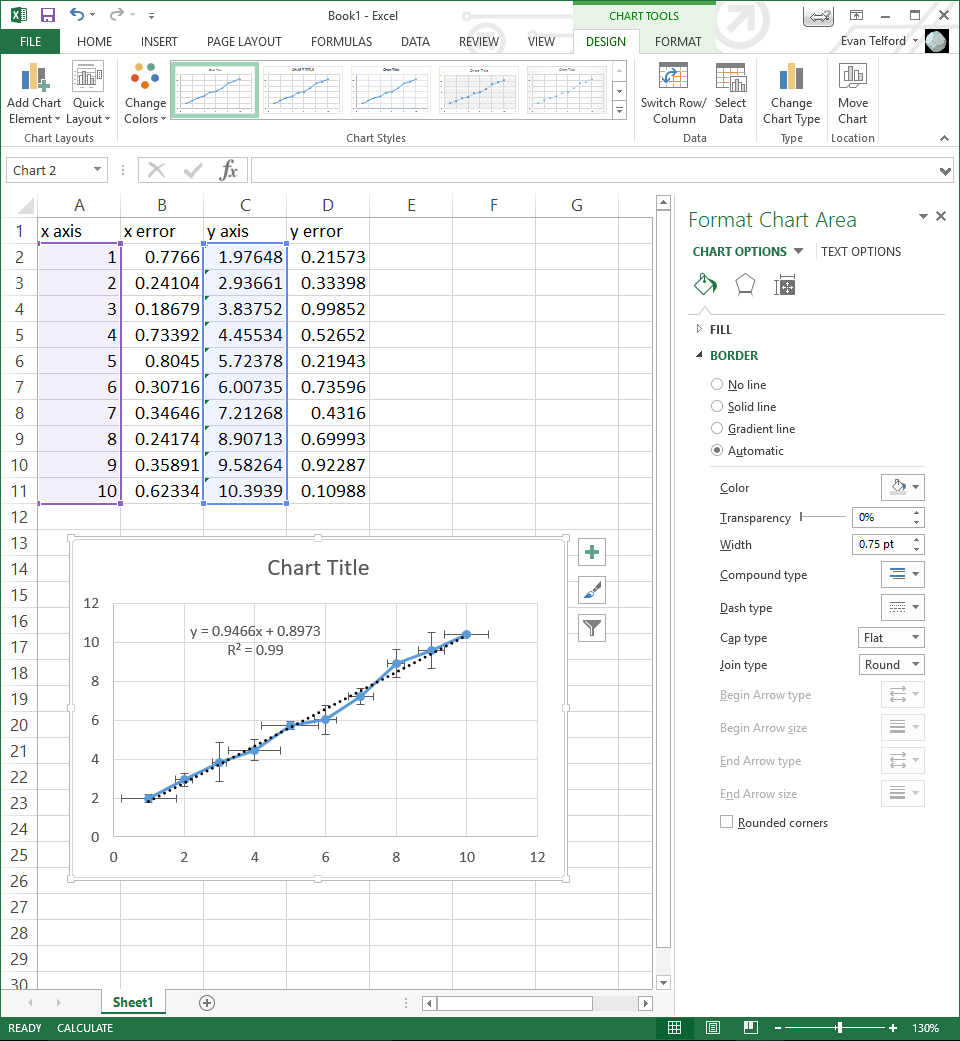
\includegraphics[height=0.4\textheight, width = 0.7\textwidth]{./Exp1-2/pic/image6.png}
\caption{Using excel to perform a linear fit and return the intercept and slope.}
\label{fig:excel3}
\end{figure}

\subsubsection{Finding Error in Slope}
\label{sec:linest}

The previous steps will help plot your data, but in order to draw conclusions, you must add uncertainty. Excel has a built in function called LINEST which finds the standard error for a linear fit. Using the same columns of data from before, the walkthrough below will help you calculate the error so you can propagate it further in the experiment.

\begin{enumerate}
\item The LINEST function is an array-type function, meaning it will output more than one number. Start, by highlighting a 2-by-3 section of empty cells (two columns, three rows).
\item With these six cells highlighted, in the input box at the top of the screen type ``= LINEST(" and add the proper arguments. The arguments should be the list of y-values, the list of x-values, TRUE, and TRUE.
For example:
$=\texttt{LINEST}(\texttt{C2:C11, A2:A11, TRUE, TRUE})$.

\item Press CONTROL+SHIFT+ENTER. \it{Note that on a Mac, this is CMD+SHIFT+ENTER.}
\end{enumerate}

Your results should have filled in that 2-by-3 section in the following way:
\begin {table}[H]
\begin{center}
\begin{tabular}{ |c | c | c |}
\hline
Slope &X Intercept \\ \hline
Error of Slope &Error of Intercept \\ \hline
$R^2$ &Error in Y \\ \hline
\end{tabular}
\caption{LINEST function output in Excel.}
\end{center}
\end{table}

\subsubsection{Helpful Commands}

Your TA will guide you through the relevant excel commands necessary for data analysis, however a list of some relevant excel commands are listed below. A list of all excel commands can be found on the \href{https://support.office.com/en-us/article/Excel-functions-alphabetical-b3944572-255d-4efb-bb96-c6d90033e188}{Microsoft Office website}\footnote{https://support.office.com/en-us/article/Excel-functions-alphabetical-b3944572-255d-4efb-bb96-c6d90033e188}

\begin{center}
\begin{tabular}{c | c}
\texttt{ABS} & Returns the absolute value of a number \\
\texttt{AVERAGE} & Computes the average of the selected data set \\
\texttt{COS} & Calculates cosine of a number\\
\texttt{DEGREES} & Converts radians to degrees \\
\texttt{EXP} & Returns e raised to the power of a given number \\
\texttt{LN} & Returns the natural logarithm of a number \\
\texttt{MEDIAN} & Finds the median of a data set \\
\texttt{MODE.SNGL} & Finds the most commonly occuring number in a data set\\
\texttt{PI} & Returns the value of pi\\
\texttt{POWER} & Returns the result of a number raised to a power\\
\texttt{SIN} & Calcualtes the sine of a number\\
\texttt{SQRT} & Calculates the square root of a number\\
\texttt{STDEV.P} & Calculates the standard deviation based on the entire population \\
\texttt{STDEV.S} & Estimates the standard deviation based on a sample \\
\texttt{SUM} & Calculates the sum of a data set\\
\texttt{TAN} & Calculates the tangent of a number
\end{tabular}
\end{center}

\subsection{Simple Pendulum}
In this experiment, we will study the dynamics of a simple pendulum. A simple pendulum is defined as a small mass (known as a pendulum bob), treated as a point mass, suspended from a thin wire considered to be massless. When displaced from equilibrium, the mass will oscillate around the equilibrium point. To analyze the mechanics of the simple pendulum, we use Newton's second law to examine the forces on the pendulum bob (see figure \ref{fig:pendulum}).
\myskip
Looking at figure \ref{fig:pendulum}, we can write down Newton's second law.
\begin{gather}
F = -mg\sin(\theta) \\
F = ml \frac{d^2}{dt^2}\theta \\
\text{using the small angle approximation} \hspace{3mm} \sin(\theta) \sim \theta \nonumber \\
-\frac{g}{l} \theta = \frac{d^2}{dt^2}\theta
\end{gather}
You may recognize equation 2.8 as the equation for simple harmonic motion. In simple harmonic motion, the object (in this case the pendulum) will oscillate about an equilibrium point with a specific frequency $f$. The frequency can be found from Newton's second law as simple harmonic motion takes the following form.
\begin{gather}
-(2\pi f)^2 \theta = \frac{d^2}{dt^2}\theta
\end{gather}
By comparison of equations 2.8 and 2.9, the frequency can be determined in terms of know parameters.
\begin{gather}
f = \frac{1}{2\pi}\sqrt{\frac{g}{l}}
\end{gather}
In experiment, we can more easily measure the period of oscillation, which is related to the frequency $\tau = 1/f$. Therefore, we also have an expression for the period of oscillation in terms of know parameters.
\begin{gather}
\tau=2\pi \sqrt{\frac{l}{g}}
\end{gather}

\begin{figure}[h]
\centering
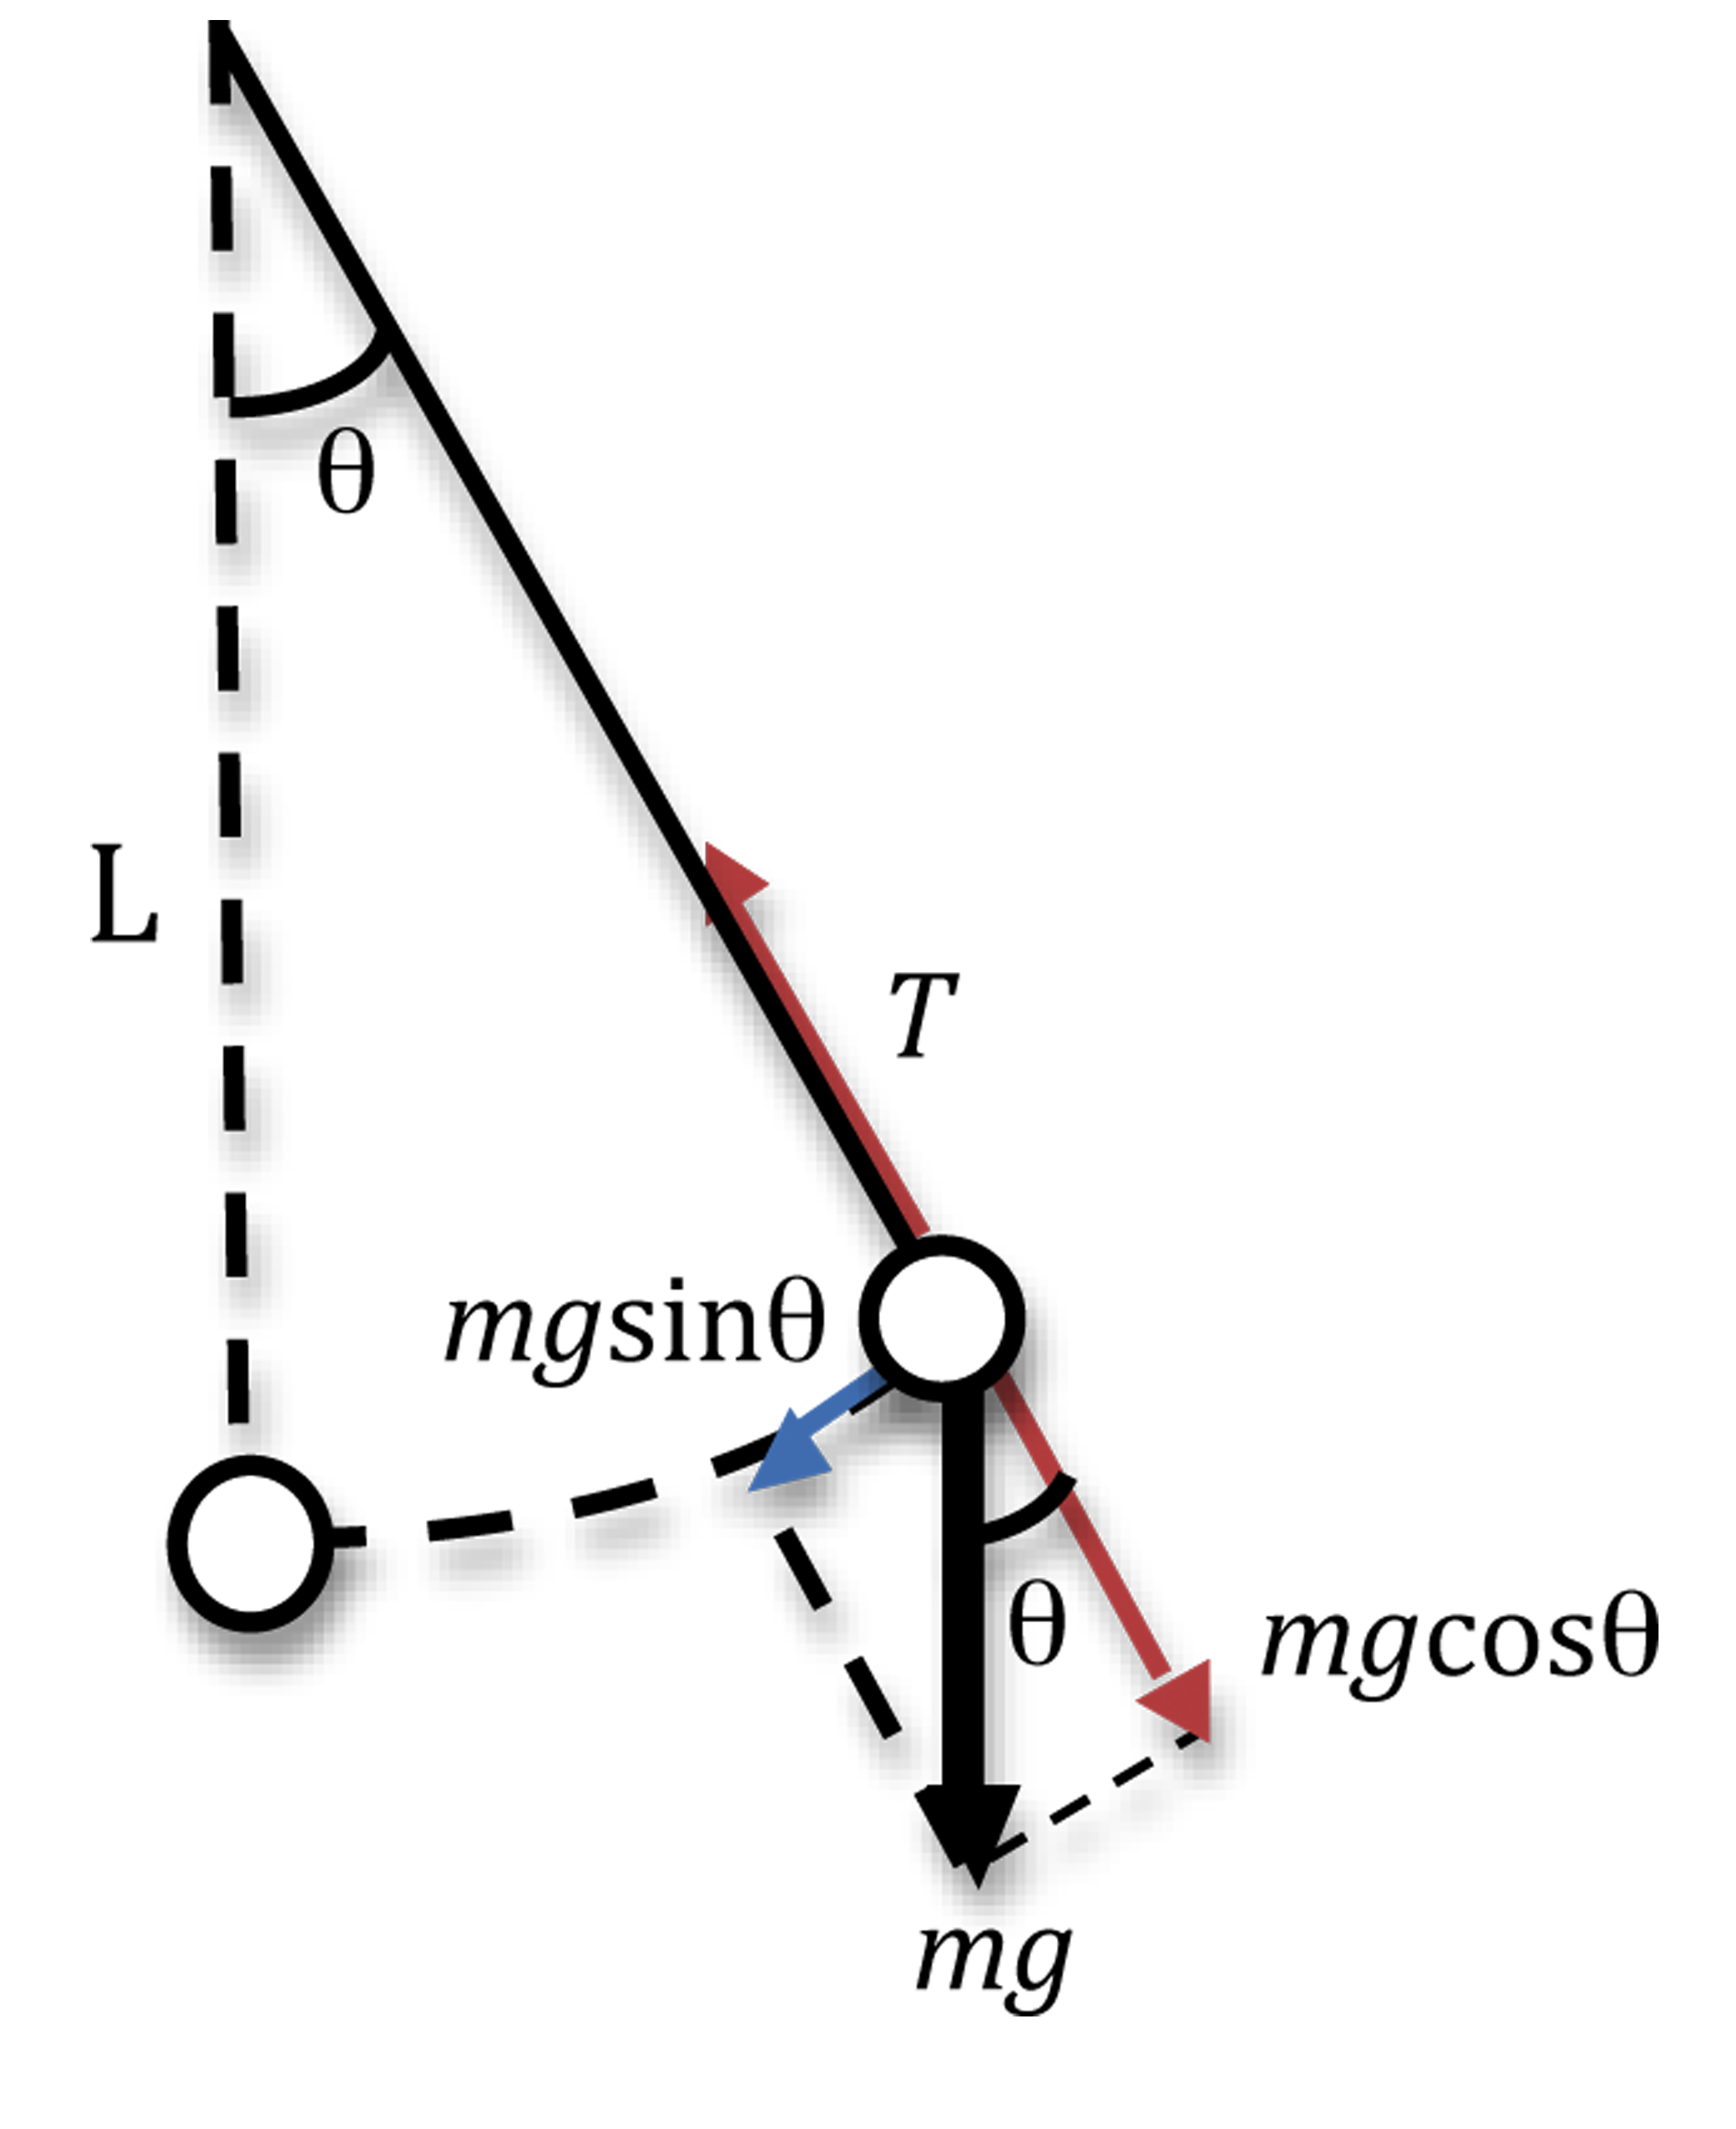
\includegraphics[width=0.5\textwidth]{./Exp1-2/pic/pendulum.png}
\caption{A free body diagram of a simple pendulum undergoing simple harmonic motion}
\label{fig:pendulum}
\end{figure}

\section{Procedure}

You will determine the gravitational constant $g$ through two methods. First, you will measure the time it takes a pendulum to swing through a full cycle, the period of oscillation, and use this to calculate the gravitational constant $g$. Second, you will measure the period for 5 different pendulum lengths and use the linear fit method to determine the gravitation constant $g$. Since a number of measurements need to be made, you may wish to perform this experiment in teams of two: one person measures the time values, the other records the results. \myskip

\begin{itemize}
\item Measurement 1: Calculation of $g$ by measuring multiple periods $\tau$.
\begin{enumerate}
\item Begin by measuring the length of the pendulum with error and recording it in your report.
\item Let the pendulum swing at some small angle (less then 15 degrees) and measure the period of the motion. Try to start and stop the stopwatch at the apex of the motion. A full period is the time it takes to travel from one maximum point to back to the same point. Take 18 measurements of the period and record the data in an excel document.
\item Use excel functions to determine the error in measured period using two methods: first, calculate the standard deviation, then estimate the error using the 2/3 method. Do the two methods give a similar error? Use standard deviation as the error in later calculations.
\item Use the following formula to determine the gravitational constant $g$ with error found by propagating uncertainties in pendulum length $l$ and period $\tau$.
\begin{gather}
 \frac{2\cdot \pi}{t} = \sqrt{\frac{g}{\ell}}
\end{gather}
\item Does your calculated value of $g$ agree with the expected value ($g=9.81 m/s^2$)?
\item What are the major sources of error in this part of the experiment?
\end{enumerate}
\item Measurement 2: Calculation of $g$ by measuring the period as a function of pendulum length.
\begin{enumerate}
\item Measure the length of the pendulum with error and record it in your report.
\item Let the pendulum swing at some small angle (less then 15 degrees) and measure the period of the motion. Try to start and stop the stopwatch at the apex of the motion. Make a single measurement of the period $\tau$.
\item repeat steps 1-2 for 5 different pendulum lengths $\ell$.
\item In excel, plot the length of the pendulum $\ell$ versus period squared $\tau^2$ with error bars on both axes. The error bars in $\ell$ and $\tau$ can be determined from the precision in the ruler/stopwatch (make sure to correctly propagate the error in squaring $\tau$).
\item Use excel to fit your plot with a line and use the generated slope to determine the gravitational constant $g$. Include error in $g$ using the LINEST method described in Section ~\ref{sec:linest}.
\item Does your calculated value of $g$ agree with the expected value?
\item What are the main sources of error in this part of the experiment?
\end{enumerate}
\end{itemize}

\newpage
\section{Applications}
You read of a certain test intended to indicate a particular kind of cancer. The test gives you a positive result for $(80 \pm 10) \%$ of all persons tested who really have this kind of cancer (true positives). But the test also gives you a positive result for $(2 \pm 1) \%$ of all healthy persons (false positives). Now you read a publication where the author performed this test on $10,000$ workers that deal with a certain chemical. The author got 400 positive samples from these workers and claims that this is strong evidence that this particular chemical enhances the development of this kind of cancer since it is known from literature that only $(1 \pm 0.5)\%$ of the population are expected to have this kind of cancer. How reliable is the claim of the author?\myskip

\noindent \underline{Numerical Answer}:

If one assumes that the 10,000 workers would mirror the average population, then there should be:
\begin{equation}
    10000 \times (0.010 \pm 0.005) = 100 \pm 50
\end{equation}
persons having this cancer. Of them, the test gives:
\begin{equation}
    (0.8 \pm 0.1) \times (100 \pm 50) = 80 \pm 50
\end{equation}
positive results (true positives).\myskip

There are then $9900 \pm 50$ persons expected not to have this kind of cancer. Of them:
\begin{equation}
    (0.02 \pm 0.01) \times (9900 \pm 50) \approx 200 \pm 100
\end{equation}
give positive results (false positives).\myskip

The total number of positives in the average population is therefore $280 \pm 150$.\myskip

So how do you judge the author's conclusion of ``strong evidences''?\myskip

If you wanted to design a new test using the same procedure but to arrive at a stronger conclusion, and you could either increase the rate of true positives or decrease the rate of wrong negatives, which would you choose?\myskip

\noindent\emph{Reference}: Paul Cutler: Problem Solving in Clinical Medicine, Chapter 5, Problem 5 (modified).

\section{Lab Preparation Examples}

\begin{enumerate}
  \item Consider a set of measurements you made of the gravitational constant $g$ on earth (in $m/s^2$). The data set is given below.
  \begin{center}
    \begin{tabular}{| c | c | c | c | c | c | c | c | c | c | c |}
      \hline
      Trial &1&2&3&4&5&6&7&8&9&10 \\ \hline
      $g (m/s^2)$&9.7&9.2&10.1&10.0&9.5&8.9&11.1&9.8&9.7&10.0 \\
      \hline
    \end{tabular}
  \end{center}
  \begin{enumerate}
    \item Calculate the mean, median, mode, and standard deviation of the data set using excel and include them in your report.
    \item Estimate the error in $g$ using the 2/3 method. How does this compare to the standard deviation?
    \item Does the mean value for $g$ agree with the expected value within error? Note the standard value of $g$  is $9.81 m/s^2$.
    \item If your mean doesn't agree (or if it hadn't agreed) with the expected value of $g$, what type of errors might have contributed to the incorrect value of $g$?
  \end{enumerate}

  \item Consider two sets of measurements in which you measured the length of a table that is known to be $1.25 m$. In the first method, you used a meter stick, so you had to measure twice. In the second method, you used a 2-meter stick, so you only had to measure once. Assume the ruler has centimeter precision.
  \begin{center}
    \begin{tabular}{ |c | c | c | c | c | c |}
      \hline
      Trial &1&2&3&4&5 \\ \hline
      Method 1, Measurement 1 ($m$) & 1.00 & 1.00 & 1.00 &1.00 &1.00 \\
      \hline
      Method 1, Measurement 2  ($m$)& 0.23 &0.21&0.25&0.26&0.24 \\
      \hline
      Method 2 ($m$)& 1.23&1.21&1.25&1.26&1.24 \\
      \hline
    \end{tabular}
  \end{center}
  \begin{enumerate}
    \item Calculate the absolute and relative uncertainties for each measurement in both trials (don't use 2/3 method or standard deviation).
    \item Which measurement is most precise (has lower relative unertainty)?
    \item Estimate the error using the 2/3 methods. How does this compare to the error you calculated in part (a).
    \item What could you conclude about making measurements with a ruler?
  \end{enumerate}

  \item Consider a measurement you made in which you counted the number of cars that passed in 1 hour on various highways in the united states. The data set containing the number of cars per hour is given in the following table.
  \begin{center}
    \begin{tabular}{|c | c | c | c | c | c | c | c | c | c | c|}
      \hline
      Trail&1&2&3&4&5&6&7&8&9&10 \\ \hline
      $N_{\text{cars}}$&523&143&496&1045&869&57&693&1150&327&87 \\
      \hline
    \end{tabular}
  \end{center}
  \begin{enumerate}
    \item Calculate the absolute error and the relative error in each measurement.
    \item Which measurement has the lowest absolute error?
    \item Which measurement has the lowest relative error?
    \item Which measurement would you say is the most precise?
    \item Calculate the rate in cars {\it{per second}} for each measurement with error.
    \item What experimental factors might contribute to the error in car rate (be creative!)?
  \end{enumerate}
\end{enumerate}
